% Original code-native footer mark, inspired by hei's running-duck identity.
% Intentionally sparse so it remains legible at roughly 8mm in grayscale.
% This is not the generated bitmap character or a claim of hand-drawn artwork.
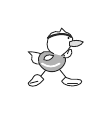
\begin{tikzpicture}[x=0.25mm,y=0.25mm,line width=0.32pt,
  line cap=round,line join=round,draw=black!85]
  % Two legs and trainers establish a running stride.
  \draw (12,10) -- (8,5);
  \path[draw,fill=white] (8,6) .. controls (6,7) and (5,6) .. (4,4)
    -- (2,2) .. controls (2,0) and (6,0) .. (8,2) -- (10,4) -- cycle;
  \draw (3,2) -- (7,3);
  \draw (18,9) -- (22,4);
  \path[draw,fill=white] (21,5) -- (19,3) .. controls (20,1) and (24,0) .. (27,1)
    .. controls (30,2) and (30,4) .. (27,4) -- (24,4) -- cycle;
  \draw (22,2) -- (27,2);
  % Tail, vest, forward wing and a clear round head.
  \path[draw,fill=white] (9,12) .. controls (5,11) and (3,13) .. (4,16)
    -- (2,18) .. controls (6,18) and (9,17) .. (11,16) -- cycle;
  \path[draw,fill=black!30] (10,18) .. controls (7,17) and (6,13) .. (9,10)
    .. controls (12,7) and (17,7) .. (20,11)
    .. controls (22,14) and (21,17) .. (18,18) -- cycle;
  \draw[white,line width=0.65pt] (9,12) .. controls (12,10) and (15,10) .. (18,12);
  \path[draw,fill=white] (20,15) .. controls (23,14) and (25,17) .. (24,19)
    .. controls (23,20) and (22,18) .. (22,17);
  \path[draw,fill=white] (15,17) .. controls (12,18) and (11,21) .. (12,24)
    .. controls (12,27) and (15,29) .. (18,28)
    -- (19,30) -- (21,28)
    .. controls (25,27) and (26,23) .. (23,20)
    .. controls (22,18) and (20,17) .. (19,16);
  \path[draw,fill=black!12] (23,23) .. controls (25,24) and (28,24) .. (30,23)
    .. controls (29,21) and (26,20) .. (23,21) -- cycle;
  \fill[black!90] (22.5,25) circle[radius=0.55];
  \draw[line width=0.75pt] (12,25) .. controls (15,27) and (21,28) .. (24,25.5);
  \path[draw,fill=white] (15,16) .. controls (12,17) and (10,16) .. (10,14)
    .. controls (12,13) and (14,14) .. (15,16);
\end{tikzpicture}
